\documentclass[]{article}
\usepackage{lmodern}
\usepackage{amssymb,amsmath}
\usepackage{ifxetex,ifluatex}
\usepackage{fixltx2e} % provides \textsubscript
\ifnum 0\ifxetex 1\fi\ifluatex 1\fi=0 % if pdftex
  \usepackage[T1]{fontenc}
  \usepackage[utf8]{inputenc}
\else % if luatex or xelatex
  \ifxetex
    \usepackage{mathspec}
  \else
    \usepackage{fontspec}
  \fi
  \defaultfontfeatures{Ligatures=TeX,Scale=MatchLowercase}
\fi
% use upquote if available, for straight quotes in verbatim environments
\IfFileExists{upquote.sty}{\usepackage{upquote}}{}
% use microtype if available
\IfFileExists{microtype.sty}{%
\usepackage{microtype}
\UseMicrotypeSet[protrusion]{basicmath} % disable protrusion for tt fonts
}{}
\usepackage[margin=1in]{geometry}
\usepackage{hyperref}
\hypersetup{unicode=true,
            pdftitle={Project 2},
            pdfauthor={Hannah Kirby},
            pdfborder={0 0 0},
            breaklinks=true}
\urlstyle{same}  % don't use monospace font for urls
\usepackage{color}
\usepackage{fancyvrb}
\newcommand{\VerbBar}{|}
\newcommand{\VERB}{\Verb[commandchars=\\\{\}]}
\DefineVerbatimEnvironment{Highlighting}{Verbatim}{commandchars=\\\{\}}
% Add ',fontsize=\small' for more characters per line
\usepackage{framed}
\definecolor{shadecolor}{RGB}{248,248,248}
\newenvironment{Shaded}{\begin{snugshade}}{\end{snugshade}}
\newcommand{\AlertTok}[1]{\textcolor[rgb]{0.94,0.16,0.16}{#1}}
\newcommand{\AnnotationTok}[1]{\textcolor[rgb]{0.56,0.35,0.01}{\textbf{\textit{#1}}}}
\newcommand{\AttributeTok}[1]{\textcolor[rgb]{0.77,0.63,0.00}{#1}}
\newcommand{\BaseNTok}[1]{\textcolor[rgb]{0.00,0.00,0.81}{#1}}
\newcommand{\BuiltInTok}[1]{#1}
\newcommand{\CharTok}[1]{\textcolor[rgb]{0.31,0.60,0.02}{#1}}
\newcommand{\CommentTok}[1]{\textcolor[rgb]{0.56,0.35,0.01}{\textit{#1}}}
\newcommand{\CommentVarTok}[1]{\textcolor[rgb]{0.56,0.35,0.01}{\textbf{\textit{#1}}}}
\newcommand{\ConstantTok}[1]{\textcolor[rgb]{0.00,0.00,0.00}{#1}}
\newcommand{\ControlFlowTok}[1]{\textcolor[rgb]{0.13,0.29,0.53}{\textbf{#1}}}
\newcommand{\DataTypeTok}[1]{\textcolor[rgb]{0.13,0.29,0.53}{#1}}
\newcommand{\DecValTok}[1]{\textcolor[rgb]{0.00,0.00,0.81}{#1}}
\newcommand{\DocumentationTok}[1]{\textcolor[rgb]{0.56,0.35,0.01}{\textbf{\textit{#1}}}}
\newcommand{\ErrorTok}[1]{\textcolor[rgb]{0.64,0.00,0.00}{\textbf{#1}}}
\newcommand{\ExtensionTok}[1]{#1}
\newcommand{\FloatTok}[1]{\textcolor[rgb]{0.00,0.00,0.81}{#1}}
\newcommand{\FunctionTok}[1]{\textcolor[rgb]{0.00,0.00,0.00}{#1}}
\newcommand{\ImportTok}[1]{#1}
\newcommand{\InformationTok}[1]{\textcolor[rgb]{0.56,0.35,0.01}{\textbf{\textit{#1}}}}
\newcommand{\KeywordTok}[1]{\textcolor[rgb]{0.13,0.29,0.53}{\textbf{#1}}}
\newcommand{\NormalTok}[1]{#1}
\newcommand{\OperatorTok}[1]{\textcolor[rgb]{0.81,0.36,0.00}{\textbf{#1}}}
\newcommand{\OtherTok}[1]{\textcolor[rgb]{0.56,0.35,0.01}{#1}}
\newcommand{\PreprocessorTok}[1]{\textcolor[rgb]{0.56,0.35,0.01}{\textit{#1}}}
\newcommand{\RegionMarkerTok}[1]{#1}
\newcommand{\SpecialCharTok}[1]{\textcolor[rgb]{0.00,0.00,0.00}{#1}}
\newcommand{\SpecialStringTok}[1]{\textcolor[rgb]{0.31,0.60,0.02}{#1}}
\newcommand{\StringTok}[1]{\textcolor[rgb]{0.31,0.60,0.02}{#1}}
\newcommand{\VariableTok}[1]{\textcolor[rgb]{0.00,0.00,0.00}{#1}}
\newcommand{\VerbatimStringTok}[1]{\textcolor[rgb]{0.31,0.60,0.02}{#1}}
\newcommand{\WarningTok}[1]{\textcolor[rgb]{0.56,0.35,0.01}{\textbf{\textit{#1}}}}
\usepackage{graphicx,grffile}
\makeatletter
\def\maxwidth{\ifdim\Gin@nat@width>\linewidth\linewidth\else\Gin@nat@width\fi}
\def\maxheight{\ifdim\Gin@nat@height>\textheight\textheight\else\Gin@nat@height\fi}
\makeatother
% Scale images if necessary, so that they will not overflow the page
% margins by default, and it is still possible to overwrite the defaults
% using explicit options in \includegraphics[width, height, ...]{}
\setkeys{Gin}{width=\maxwidth,height=\maxheight,keepaspectratio}
\IfFileExists{parskip.sty}{%
\usepackage{parskip}
}{% else
\setlength{\parindent}{0pt}
\setlength{\parskip}{6pt plus 2pt minus 1pt}
}
\setlength{\emergencystretch}{3em}  % prevent overfull lines
\providecommand{\tightlist}{%
  \setlength{\itemsep}{0pt}\setlength{\parskip}{0pt}}
\setcounter{secnumdepth}{0}
% Redefines (sub)paragraphs to behave more like sections
\ifx\paragraph\undefined\else
\let\oldparagraph\paragraph
\renewcommand{\paragraph}[1]{\oldparagraph{#1}\mbox{}}
\fi
\ifx\subparagraph\undefined\else
\let\oldsubparagraph\subparagraph
\renewcommand{\subparagraph}[1]{\oldsubparagraph{#1}\mbox{}}
\fi

%%% Use protect on footnotes to avoid problems with footnotes in titles
\let\rmarkdownfootnote\footnote%
\def\footnote{\protect\rmarkdownfootnote}

%%% Change title format to be more compact
\usepackage{titling}

% Create subtitle command for use in maketitle
\providecommand{\subtitle}[1]{
  \posttitle{
    \begin{center}\large#1\end{center}
    }
}

\setlength{\droptitle}{-2em}

  \title{Project 2}
    \pretitle{\vspace{\droptitle}\centering\huge}
  \posttitle{\par}
    \author{Hannah Kirby}
    \preauthor{\centering\large\emph}
  \postauthor{\par}
      \predate{\centering\large\emph}
  \postdate{\par}
    \date{11/18/2019}


\begin{document}
\maketitle

\textbf{\emph{Modeling, Testing, and Predicting}}

\begin{Shaded}
\begin{Highlighting}[]
\KeywordTok{library}\NormalTok{(}\StringTok{"boot"}\NormalTok{)}
\KeywordTok{library}\NormalTok{(}\StringTok{"tidyverse"}\NormalTok{)}
\end{Highlighting}
\end{Shaded}

\begin{verbatim}
## Warning in as.POSIXlt.POSIXct(Sys.time()): unknown timezone 'zone/tz/2019c.
## 1.0/zoneinfo/America/Chicago'
\end{verbatim}

\begin{verbatim}
## -- Attaching packages ------------------------------------------------------------ tidyverse 1.2.1 --
\end{verbatim}

\begin{verbatim}
## v ggplot2 3.2.1     v purrr   0.3.2
## v tibble  2.1.3     v dplyr   0.8.3
## v tidyr   1.0.0     v stringr 1.4.0
## v readr   1.1.1     v forcats 0.4.0
\end{verbatim}

\begin{verbatim}
## Warning: package 'readr' was built under R version 3.3.2
\end{verbatim}

\begin{verbatim}
## -- Conflicts --------------------------------------------------------------- tidyverse_conflicts() --
## x dplyr::filter() masks stats::filter()
## x dplyr::lag()    masks stats::lag()
\end{verbatim}

\begin{Shaded}
\begin{Highlighting}[]
\KeywordTok{library}\NormalTok{(sandwich)}
\KeywordTok{library}\NormalTok{(lmtest)}
\end{Highlighting}
\end{Shaded}

\begin{verbatim}
## Warning: package 'lmtest' was built under R version 3.3.2
\end{verbatim}

\begin{verbatim}
## Loading required package: zoo
\end{verbatim}

\begin{verbatim}
## 
## Attaching package: 'zoo'
\end{verbatim}

\begin{verbatim}
## The following objects are masked from 'package:base':
## 
##     as.Date, as.Date.numeric
\end{verbatim}

\begin{Shaded}
\begin{Highlighting}[]
\KeywordTok{head}\NormalTok{(melanoma)}
\end{Highlighting}
\end{Shaded}

\begin{verbatim}
##   time status sex age year thickness ulcer
## 1   10      3   1  76 1972      6.76     1
## 2   30      3   1  56 1968      0.65     0
## 3   35      2   1  41 1977      1.34     0
## 4   99      3   0  71 1968      2.90     0
## 5  185      1   1  52 1965     12.08     1
## 6  204      1   1  28 1971      4.84     1
\end{verbatim}

\begin{Shaded}
\begin{Highlighting}[]
\NormalTok{melanoma<-melanoma}
\end{Highlighting}
\end{Shaded}

\emph{This dataset contains information about melanoma cases in
Connecticut from the years 1936-1972. There are 205 observatins and 7
variables. Variables included in this dataset include survival time in
days since the operation, survival status, gender, age, year of the
operation, thickness of the melanoma, and presence or absence of an
ulcer in which 1=ulcer and 0=no ulcer. As for survival status, survival
is ranked 1-3, in wich 1=died from melanoma, 2=still alive, and 3=death
by other causes. For analysis in this project, I am more concerned with
1 and 2, so I will be omiting 3 from the survival data.}

\begin{Shaded}
\begin{Highlighting}[]
\NormalTok{melanoma<-}\StringTok{ }\NormalTok{melanoma}\OperatorTok\StringTok{ }\KeywordTok{filter}\NormalTok{(status}\OperatorTok{<}\DecValTok{3}\NormalTok{)}
\NormalTok{melanoma<-melanoma}\OperatorTok\StringTok{ }\KeywordTok{mutate}\NormalTok{(}\DataTypeTok{y=}\KeywordTok{ifelse}\NormalTok{(melanoma}\OperatorTok{$}\NormalTok{status}\OperatorTok{==}\DecValTok{2}\NormalTok{,}\DecValTok{1}\NormalTok{,}\DecValTok{0}\NormalTok{))}
\end{Highlighting}
\end{Shaded}

\emph{After removing the rows where status=3, the data is left with 191
observations. In addition to this, I am making the status variable into
another variable y, in which survival (which is represented by a 2 in
the status variable) is represented by 1, and death from melanoma (which
is represented by a 1 in the status variable) is represented by a 0.
This is the binomial variable for the dataset.}

\textbf{MANOVA}

\begin{Shaded}
\begin{Highlighting}[]
\KeywordTok{ggplot}\NormalTok{(melanoma, }\KeywordTok{aes}\NormalTok{(}\DataTypeTok{x =}\NormalTok{age , }\DataTypeTok{y =}\NormalTok{ thickness)) }\OperatorTok{+}\KeywordTok{geom_point}\NormalTok{(}\DataTypeTok{alpha =} \FloatTok{.5}\NormalTok{) }\OperatorTok{+}\StringTok{ }\KeywordTok{geom_density_2d}\NormalTok{(}\DataTypeTok{h=}\DecValTok{2}\NormalTok{) }\OperatorTok{+}\StringTok{ }\KeywordTok{expand_limits}\NormalTok{(}\DataTypeTok{x=}\KeywordTok{c}\NormalTok{(}\DecValTok{0}\NormalTok{,}\DecValTok{100}\NormalTok{), }\DataTypeTok{y=}\KeywordTok{c}\NormalTok{(}\DecValTok{0}\NormalTok{, }\DecValTok{25}\NormalTok{)) }\OperatorTok{+}\StringTok{ }\KeywordTok{coord_fixed}\NormalTok{(}\DecValTok{2}\NormalTok{) }\OperatorTok{+}\StringTok{ }\KeywordTok{facet_wrap}\NormalTok{(}\OperatorTok{~}\NormalTok{sex) }
\end{Highlighting}
\end{Shaded}

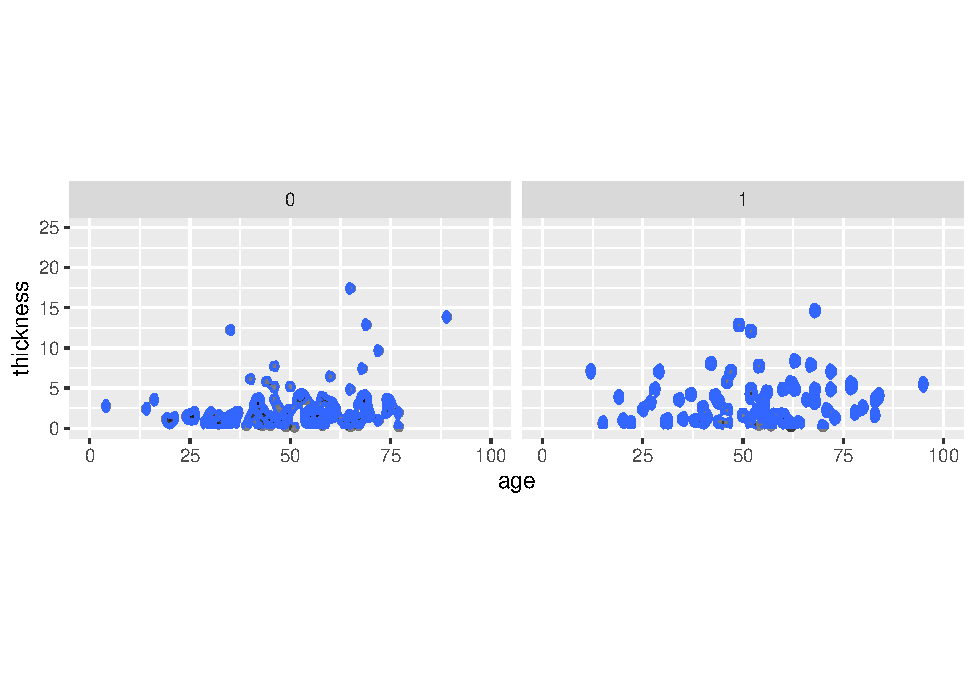
\includegraphics{Project2_files/figure-latex/unnamed-chunk-3-1.pdf}
\emph{By eyeballing this graph, it seems to have mulitvariate normality,
which is an importatn assumption of a MANOVA test. Now we can move on an
run the MANOVA test. } \emph{Null Hypothesis: for age and thickness,
mean of each sex is equal.} \emph{Alternate Hypothesis: for one of these
variables, at least one species mean is different.}

\begin{Shaded}
\begin{Highlighting}[]
\NormalTok{man1<-}\KeywordTok{manova}\NormalTok{(}\KeywordTok{cbind}\NormalTok{(age, thickness)}\OperatorTok{~}\NormalTok{sex, }\DataTypeTok{data=}\NormalTok{melanoma)}
\KeywordTok{summary}\NormalTok{(man1)}
\end{Highlighting}
\end{Shaded}

\begin{verbatim}
##            Df   Pillai approx F num Df den Df  Pr(>F)  
## sex         1 0.030306   2.9378      2    188 0.05542 .
## Residuals 189                                          
## ---
## Signif. codes:  0 '***' 0.001 '**' 0.01 '*' 0.05 '.' 0.1 ' ' 1
\end{verbatim}

\emph{The results of the MANOVA show that the p-value is greater than
0.05, meaning that we fail to reject the null hypothesis. Therefore, it
is true that for the variables age and thickness, the mean of each sex
is equal.}

\emph{If my MANOVA test would have peoduced significant results, I would
have conducted two different ANOVA tests-one for sex and thickness, and
one for sex and age. In this case, no t-tests are required because the
categorical predictor only had two levels, therefore the total number of
tests that would have been conducted is 3. }

\begin{Shaded}
\begin{Highlighting}[]
\FloatTok{.05}\OperatorTok{/}\DecValTok{3}
\end{Highlighting}
\end{Shaded}

\begin{verbatim}
## [1] 0.01666667
\end{verbatim}

\emph{Here is the calulation for the probability of at least one type I
error. It is essentially alpha (which is 0.05) divided by the total
number of tests (3-explained above). Therefore the probability is
0.01667.}

\textbf{RANDOMIZATION TEST} \emph{I am going to conduct a randomization
test for the status and thickness variables.} \emph{Null Hypothesis:
Mean thickness is the same between males and females.} \emph{Alternate
Hypothesis: Mean thickness is significantly different between males and
females.}

\begin{Shaded}
\begin{Highlighting}[]
\NormalTok{rand_dist<-}\KeywordTok{vector}\NormalTok{()}
\ControlFlowTok{for}\NormalTok{(i }\ControlFlowTok{in} \DecValTok{1}\OperatorTok{:}\DecValTok{5000}\NormalTok{)\{}
\NormalTok{new<-}\KeywordTok{data.frame}\NormalTok{(}\DataTypeTok{thickness=}\KeywordTok{sample}\NormalTok{(melanoma}\OperatorTok{$}\NormalTok{thickness),}\DataTypeTok{status=}\NormalTok{melanoma}\OperatorTok{$}\NormalTok{y)}
\NormalTok{rand_dist[i]<-}\KeywordTok{mean}\NormalTok{(new[new}\OperatorTok{$}\NormalTok{status}\OperatorTok{==}\DecValTok{0}\NormalTok{,]}\OperatorTok{$}\NormalTok{thickness)}\OperatorTok{-}
\StringTok{ }\KeywordTok{mean}\NormalTok{(new[new}\OperatorTok{$}\NormalTok{status}\OperatorTok{==}\DecValTok{1}\NormalTok{,]}\OperatorTok{$}\NormalTok{thickness)\}}
\KeywordTok{hist}\NormalTok{(rand_dist,}\DataTypeTok{main=}\StringTok{""}\NormalTok{,}\DataTypeTok{ylab=}\StringTok{""}\NormalTok{); }\KeywordTok{abline}\NormalTok{(}\DataTypeTok{v =} \FloatTok{-1.2476}\NormalTok{,}\DataTypeTok{col=}\StringTok{"red"}\NormalTok{)}
\end{Highlighting}
\end{Shaded}

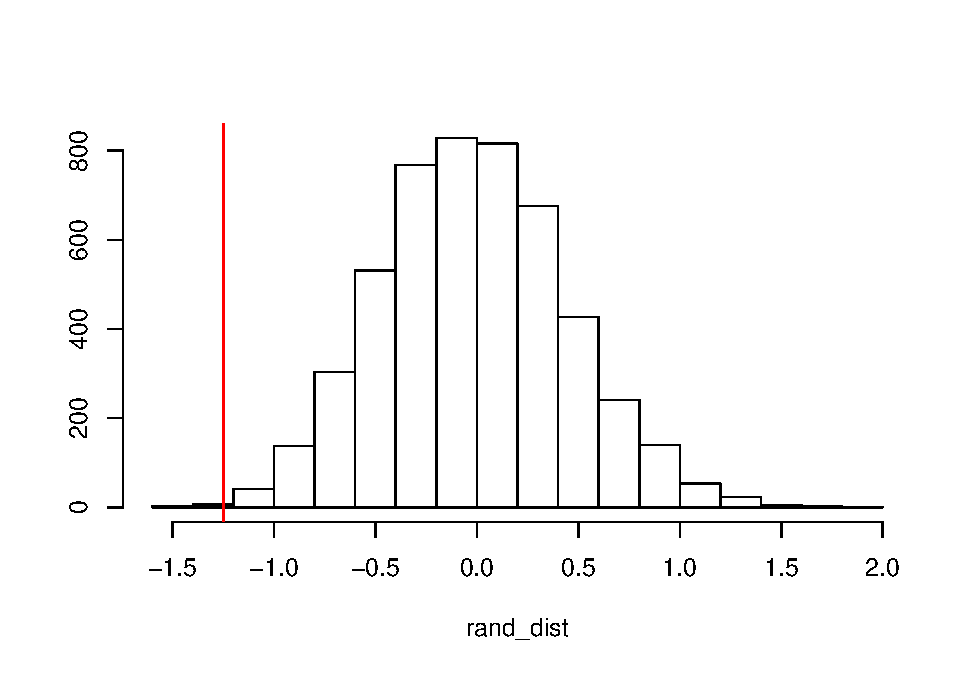
\includegraphics{Project2_files/figure-latex/unnamed-chunk-6-1.pdf}

\begin{Shaded}
\begin{Highlighting}[]
\NormalTok{melanoma}\OperatorTok\KeywordTok{group_by}\NormalTok{(y)}\OperatorTok\KeywordTok{summarize}\NormalTok{(}\DataTypeTok{s=}\KeywordTok{sd}\NormalTok{(thickness))}\OperatorTok\KeywordTok{summarize}\NormalTok{(}\KeywordTok{diff}\NormalTok{(s))}
\end{Highlighting}
\end{Shaded}

\begin{verbatim}
## # A tibble: 1 x 1
##   `diff(s)`
##       <dbl>
## 1     -1.25
\end{verbatim}

\begin{Shaded}
\begin{Highlighting}[]
\KeywordTok{mean}\NormalTok{(rand_dist}\OperatorTok{<}\StringTok{ }\FloatTok{-1.247643}\NormalTok{)}\OperatorTok{*}\DecValTok{2}
\end{Highlighting}
\end{Shaded}

\begin{verbatim}
## [1] 0.0012
\end{verbatim}

\begin{Shaded}
\begin{Highlighting}[]
\KeywordTok{t.test}\NormalTok{(}\DataTypeTok{data=}\NormalTok{melanoma, thickness}\OperatorTok{~}\NormalTok{y)}
\end{Highlighting}
\end{Shaded}

\begin{verbatim}
## 
##  Welch Two Sample t-test
## 
## data:  thickness by y
## t = 4.0182, df = 76.95, p-value = 0.0001355
## alternative hypothesis: true difference in means is not equal to 0
## 95 percent confidence interval:
##  1.042337 3.090366
## sample estimates:
## mean in group 0 mean in group 1 
##        4.311053        2.244701
\end{verbatim}

\emph{Here I conducted a simple randomization test for the difference in
standard deviations. I used the two variables of status (for which I
actually used the y variable) and thickness. The result of this test was
a p-value of 0.0028 (less than 0.05), therefore the null hypothesis is
rejected. This means that there is a significant difference in mean
thickness among males and females. In addition to this, I conducted a
quick t-test on the data just to compare. This test resulted in a
p-value of 0.00014, which just backs up the fact that there is a
difference in mean thickness across the sex variable. Lastly, the
histogram here shows the random distribution, and the red line indicates
a standard deviation.}

\textbf{LINEAR REGRESSION MODEL}

\begin{Shaded}
\begin{Highlighting}[]
\NormalTok{melanoma}\OperatorTok{$}\StringTok{ }\NormalTok{age_c<-(melanoma}\OperatorTok{$}\NormalTok{age}\OperatorTok{-}\KeywordTok{mean}\NormalTok{(melanoma}\OperatorTok{$}\NormalTok{age))}

\NormalTok{fit<-}\KeywordTok{lm}\NormalTok{(thickness}\OperatorTok{~}\StringTok{ }\NormalTok{sex }\OperatorTok{*}\StringTok{ }\NormalTok{age_c, }\DataTypeTok{data=}\NormalTok{melanoma)}
\KeywordTok{summary}\NormalTok{(fit)}
\end{Highlighting}
\end{Shaded}

\begin{verbatim}
## 
## Call:
## lm(formula = thickness ~ sex * age_c, data = melanoma)
## 
## Residuals:
##     Min      1Q  Median      3Q     Max 
## -3.6434 -1.7836 -0.6720  0.9413 14.3417 
## 
## Coefficients:
##             Estimate Std. Error t value Pr(>|t|)    
## (Intercept)  2.51851    0.26017   9.680   <2e-16 ***
## sex          0.94530    0.42427   2.228   0.0271 *  
## age_c        0.04153    0.01648   2.520   0.0126 *  
## sex:age_c   -0.02315    0.02495  -0.928   0.3547    
## ---
## Signif. codes:  0 '***' 0.001 '**' 0.01 '*' 0.05 '.' 0.1 ' ' 1
## 
## Residual standard error: 2.833 on 187 degrees of freedom
## Multiple R-squared:  0.0652, Adjusted R-squared:  0.0502 
## F-statistic: 4.347 on 3 and 187 DF,  p-value: 0.005482
\end{verbatim}

\emph{Here, I centered the age variable by subtracting the mean of the
age variable from each value in order to prepare it for a linear
regression model. The linear regression model prouced a coefficient for
each variable tested in reference to another variable, and in this case
the reference was female sex. Here are the explanations for the
coefficients:} \emph{0.945 is the predicted value of thickness when age
is 0 and sex is male.} \emph{0.042 is the predicted value of thickness
when sex is 0.} \emph{The predicted value of thickness for the
interaction is -0.023.}

\begin{Shaded}
\begin{Highlighting}[]
\NormalTok{melanoma}\OperatorTok{$}\NormalTok{sex<-}\StringTok{ }\KeywordTok{as.character}\NormalTok{(}\KeywordTok{as.numeric}\NormalTok{(melanoma}\OperatorTok{$}\NormalTok{sex))}
\KeywordTok{ggplot}\NormalTok{(}\DataTypeTok{data=}\NormalTok{melanoma, }\KeywordTok{aes}\NormalTok{(}\DataTypeTok{x =}\NormalTok{ age, }\DataTypeTok{y =}\NormalTok{ thickness,}\DataTypeTok{color=}\NormalTok{sex )) }\OperatorTok{+}\StringTok{ }\KeywordTok{geom_point}\NormalTok{() }\OperatorTok{+}\StringTok{ }\KeywordTok{geom_smooth}\NormalTok{(}\DataTypeTok{method=}\StringTok{"lm"}\NormalTok{, }\DataTypeTok{se=}\OtherTok{FALSE}\NormalTok{, }\DataTypeTok{fullrange=}\OtherTok{TRUE}\NormalTok{)}
\end{Highlighting}
\end{Shaded}

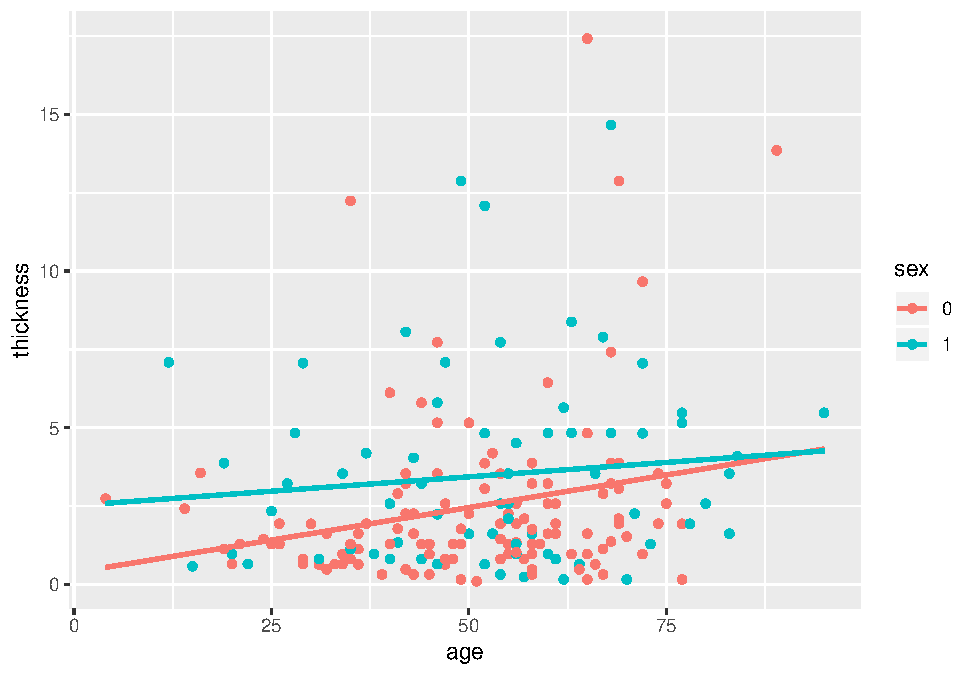
\includegraphics{Project2_files/figure-latex/unnamed-chunk-8-1.pdf}
\emph{This graph shows the regression results. }

\begin{Shaded}
\begin{Highlighting}[]
\NormalTok{resids<-fit}\OperatorTok{$}\NormalTok{residuals}
\NormalTok{fitvals<-fit}\OperatorTok{$}\NormalTok{fitted.values}
\KeywordTok{ggplot}\NormalTok{()}\OperatorTok{+}\KeywordTok{geom_point}\NormalTok{(}\KeywordTok{aes}\NormalTok{(fitvals,resids))}\OperatorTok{+}\KeywordTok{geom_hline}\NormalTok{(}\DataTypeTok{yintercept=}\DecValTok{0}\NormalTok{, }\DataTypeTok{color=}\StringTok{'red'}\NormalTok{)}
\end{Highlighting}
\end{Shaded}

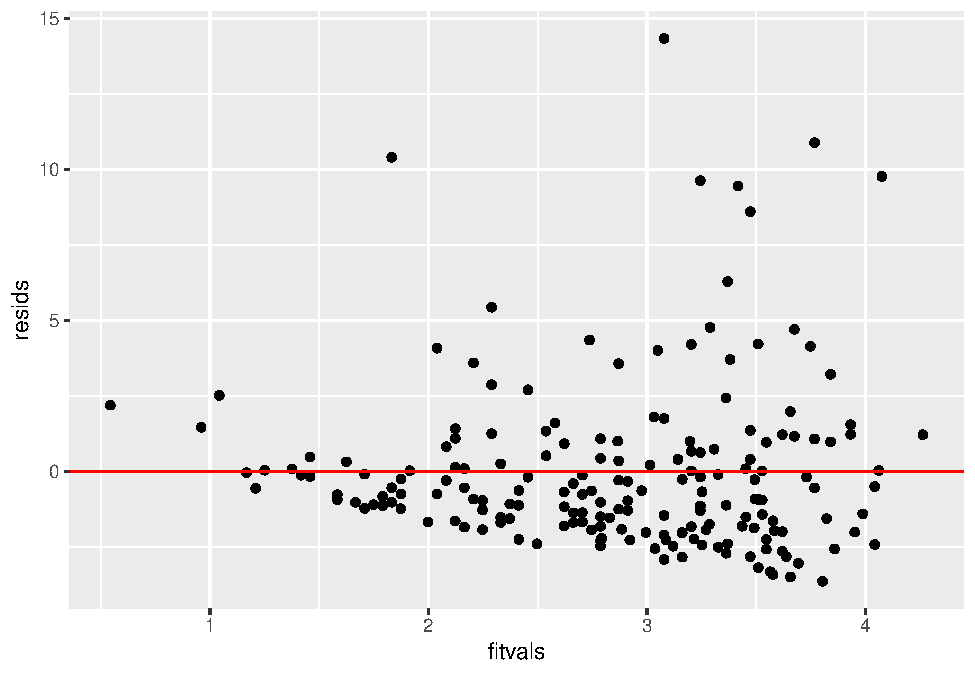
\includegraphics{Project2_files/figure-latex/unnamed-chunk-9-1.pdf}

\begin{Shaded}
\begin{Highlighting}[]
\KeywordTok{ggplot}\NormalTok{()}\OperatorTok{+}\KeywordTok{geom_histogram}\NormalTok{(}\KeywordTok{aes}\NormalTok{(resids),}\DataTypeTok{bins=}\DecValTok{20}\NormalTok{)}
\end{Highlighting}
\end{Shaded}

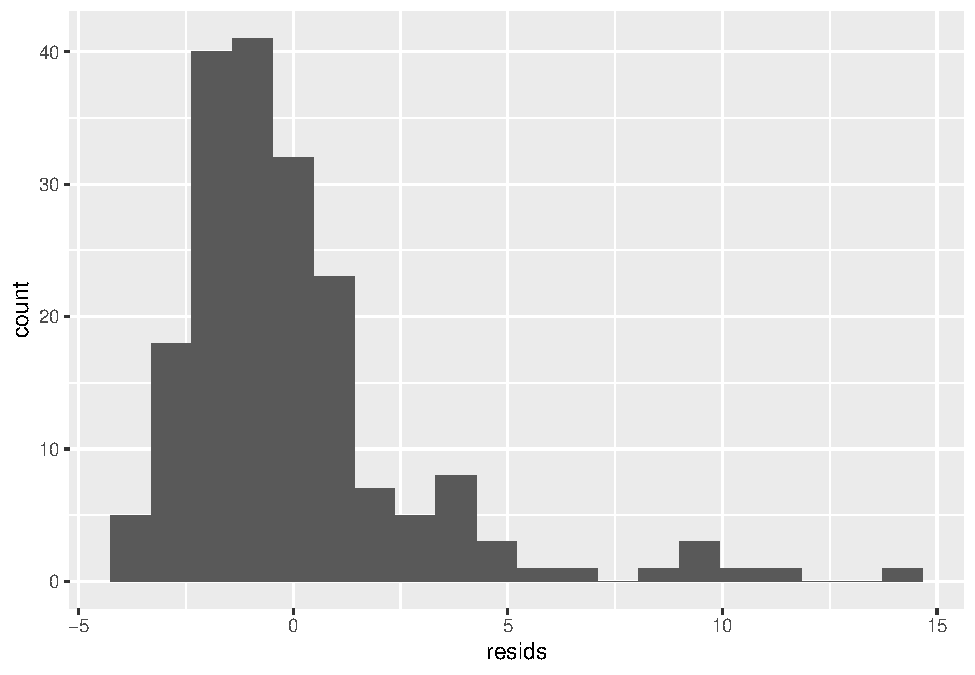
\includegraphics{Project2_files/figure-latex/unnamed-chunk-9-2.pdf}

\begin{Shaded}
\begin{Highlighting}[]
\KeywordTok{ggplot}\NormalTok{()}\OperatorTok{+}\KeywordTok{geom_qq}\NormalTok{(}\KeywordTok{aes}\NormalTok{(}\DataTypeTok{sample=}\NormalTok{resids))}\OperatorTok{+}\KeywordTok{geom_qq_line}\NormalTok{(}\KeywordTok{aes}\NormalTok{(}\DataTypeTok{sample=}\NormalTok{resids), }\DataTypeTok{color=}\StringTok{'red'}\NormalTok{)}
\end{Highlighting}
\end{Shaded}

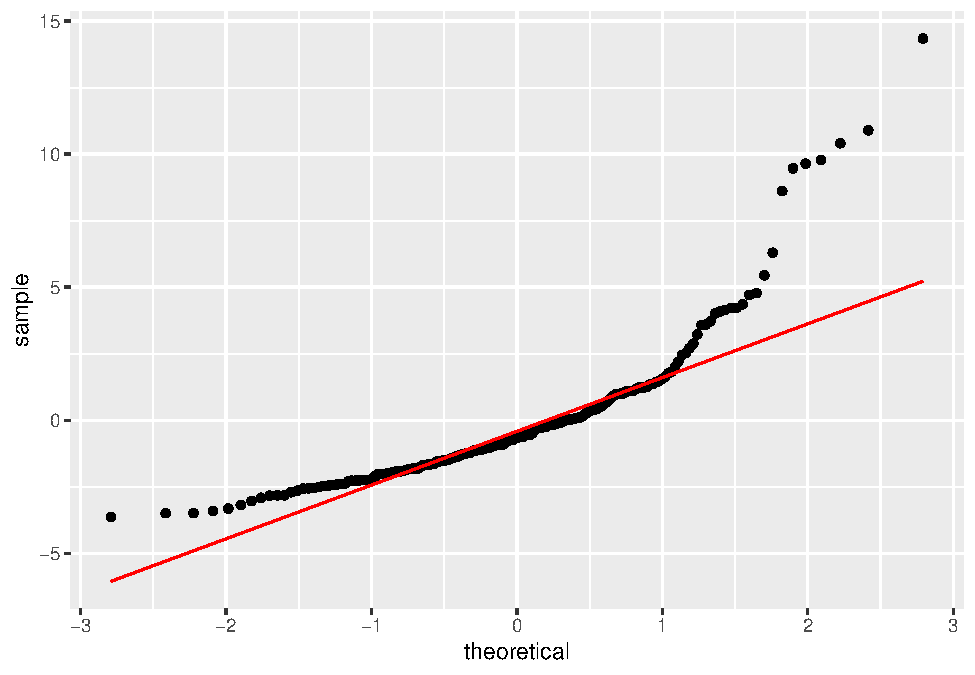
\includegraphics{Project2_files/figure-latex/unnamed-chunk-9-3.pdf}

\begin{Shaded}
\begin{Highlighting}[]
\KeywordTok{library}\NormalTok{(sandwich); }\KeywordTok{library}\NormalTok{(lmtest)}
\KeywordTok{bptest}\NormalTok{(fit)}
\end{Highlighting}
\end{Shaded}

\begin{verbatim}
## 
##  studentized Breusch-Pagan test
## 
## data:  fit
## BP = 5.0434, df = 3, p-value = 0.1686
\end{verbatim}

\emph{This series of graphs and the Breusch-Pagan test are to check the
assumptions of linearity, normality, and homoskedaticity that are
necessary conditions for linear regression models. The first graph shows
that linearity looks good. The second and third graphs show that the
normality look okay. Lastly, the Breusch-Pagan test resulted in a
non-significant p-value, meaning that we accept the null hypothesis of
this test, which is homoskedasticity. All assumptions pass.}

\begin{Shaded}
\begin{Highlighting}[]
\KeywordTok{coeftest}\NormalTok{(fit, }\DataTypeTok{vcov=}\KeywordTok{vcovHC}\NormalTok{(fit))}
\end{Highlighting}
\end{Shaded}

\begin{verbatim}
## 
## t test of coefficients:
## 
##              Estimate Std. Error t value Pr(>|t|)    
## (Intercept)  2.518512   0.260288  9.6759  < 2e-16 ***
## sex          0.945297   0.446320  2.1180  0.03550 *  
## age_c        0.041535   0.020129  2.0634  0.04046 *  
## sex:age_c   -0.023155   0.026467 -0.8749  0.38278    
## ---
## Signif. codes:  0 '***' 0.001 '**' 0.01 '*' 0.05 '.' 0.1 ' ' 1
\end{verbatim}

\emph{Re-conducting the regression with robust standard errors results
in the same significant variable coefficients as the original linear
regression model. The sex (male) and centered age variables are still
signifint and the coefficients are still the same values. }

\begin{Shaded}
\begin{Highlighting}[]
\NormalTok{(}\KeywordTok{sum}\NormalTok{((melanoma}\OperatorTok{$}\NormalTok{thicknesss}\OperatorTok{-}\KeywordTok{mean}\NormalTok{(melanoma}\OperatorTok{$}\NormalTok{thickness))}\OperatorTok{^}\DecValTok{2}\NormalTok{))}\OperatorTok{-}\NormalTok{(}\KeywordTok{sum}\NormalTok{(fit}\OperatorTok{$}\NormalTok{residuals}\OperatorTok{^}\DecValTok{2}\NormalTok{))}\OperatorTok{/}\NormalTok{(}\KeywordTok{sum}\NormalTok{((melanoma}\OperatorTok{$}\NormalTok{thickness}\OperatorTok{-}\KeywordTok{mean}\NormalTok{(melanoma}\OperatorTok{$}\NormalTok{thickness))}\OperatorTok{^}\DecValTok{2}\NormalTok{))}
\end{Highlighting}
\end{Shaded}

\begin{verbatim}
## [1] -0.934804
\end{verbatim}

\emph{The explains 93.5\% of the variation in the outcome.}

\textbf{LINEAR REGRESSION MODEL WITH BOOTSTRAPPED STANDARD ERRORS}

\begin{Shaded}
\begin{Highlighting}[]
\NormalTok{samp_distn<-}\KeywordTok{replicate}\NormalTok{(}\DecValTok{5000}\NormalTok{, \{}
\NormalTok{ boot_dat<-melanoma[}\KeywordTok{sample}\NormalTok{(}\KeywordTok{nrow}\NormalTok{(melanoma),}\DataTypeTok{replace=}\OtherTok{TRUE}\NormalTok{),]}
\NormalTok{ fit<-}\KeywordTok{lm}\NormalTok{(thickness}\OperatorTok{~}\StringTok{ }\NormalTok{sex }\OperatorTok{*}\StringTok{ }\NormalTok{age_c, }\DataTypeTok{data=}\NormalTok{boot_dat)}
 \KeywordTok{coef}\NormalTok{(fit)}
\NormalTok{\})}
\NormalTok{samp_distn}\OperatorTok\NormalTok{t}\OperatorTok\NormalTok{as.data.frame}\OperatorTok\KeywordTok{summarize_all}\NormalTok{(sd)}
\end{Highlighting}
\end{Shaded}

\begin{verbatim}
##   (Intercept)      sex1      age_c sex1:age_c
## 1   0.2563555 0.4368779 0.01963185 0.02588264
\end{verbatim}

\emph{The linear regression model with bootstrapped standard errors
produced different results than the initial linear regression model and
the linear regression with robust standard errors (which produced the
same result). All of the coefficients in this model are smaller than the
coefficients in the original models, which means that the slopes for
each variable when the other variables are held constant decreased
overall, pointing to a less sensitive model.}

\textbf{LOGISTIC REGRESSION}

\begin{Shaded}
\begin{Highlighting}[]
\CommentTok{#fit1<-glm(y~thickness + age,data=melanoma,family=binomial)}
\CommentTok{#coeftest(fit1)}

\CommentTok{#0 age and 0 thickness}
\KeywordTok{exp}\NormalTok{(}\FloatTok{2.208}\NormalTok{)}
\end{Highlighting}
\end{Shaded}

\begin{verbatim}
## [1] 9.097503
\end{verbatim}

\begin{Shaded}
\begin{Highlighting}[]
\CommentTok{#1 thickness and 0 age}
\KeywordTok{exp}\NormalTok{(}\FloatTok{2.208} \OperatorTok{+-}\FloatTok{0.238}\NormalTok{)}
\end{Highlighting}
\end{Shaded}

\begin{verbatim}
## [1] 7.170676
\end{verbatim}

\begin{Shaded}
\begin{Highlighting}[]
\CommentTok{#1 age and 0 thickness}
\KeywordTok{exp}\NormalTok{(}\FloatTok{2.208}\OperatorTok{+-}\FloatTok{0.012}\NormalTok{)}
\end{Highlighting}
\end{Shaded}

\begin{verbatim}
## [1] 8.988986
\end{verbatim}

\emph{This logistic regression model produced very descriptive
coefficients. For 0 age and 0 thickness (which doesnt make much sense),
the odds of survival after a melanoma surgery is 9.098. For 1 thickness
and 0 age, the odds of survival is 7.171. For 1 age and 0 thickness, the
odds of survival is 8.989.}

\begin{Shaded}
\begin{Highlighting}[]
\CommentTok{#melanoma$prob<-predict(fit1,type="response")}
\CommentTok{#table(truth=melanoma$y, predict=as.numeric(melanoma$prob>.5))%>%addmargins}
\end{Highlighting}
\end{Shaded}

\emph{This is a confusion matrix for the logistic regression
predictions. There are 125 true positives, 9 true negatives, 47 false
positives, and 10 false negatives.}

\begin{Shaded}
\begin{Highlighting}[]
\CommentTok{#accuracy}
\NormalTok{(}\DecValTok{10}\OperatorTok{+}\DecValTok{125}\NormalTok{)}\OperatorTok{/}\DecValTok{191}
\end{Highlighting}
\end{Shaded}

\begin{verbatim}
## [1] 0.7068063
\end{verbatim}

\begin{Shaded}
\begin{Highlighting}[]
\CommentTok{#tnr}
\DecValTok{10}\OperatorTok{/}\DecValTok{57}
\end{Highlighting}
\end{Shaded}

\begin{verbatim}
## [1] 0.1754386
\end{verbatim}

\begin{Shaded}
\begin{Highlighting}[]
\CommentTok{#tpr}
\DecValTok{125}\OperatorTok{/}\DecValTok{134}
\end{Highlighting}
\end{Shaded}

\begin{verbatim}
## [1] 0.9328358
\end{verbatim}

\begin{Shaded}
\begin{Highlighting}[]
\CommentTok{#ppv}
\DecValTok{125}\OperatorTok{/}\DecValTok{172}
\end{Highlighting}
\end{Shaded}

\begin{verbatim}
## [1] 0.7267442
\end{verbatim}

\emph{The accuracy of this logistic regression model is 0.7068, the
specificity is 0.1754, the sensitivity is 0.9328, and the recall is
0.7267.}

\begin{Shaded}
\begin{Highlighting}[]
\CommentTok{#melanoma$y<- as.factor(as.numeric(melanoma$sex))}

\CommentTok{#melanoma$logit<-predict(fit1)}
\CommentTok{#melanoma$outcome <-factor(melanoma$y,levels=c("survived","died"))}
\CommentTok{#ggplot(data=melanoma,aes(logit, fill=melanoma$y))+geom_density(alpha=.3)+}
  \CommentTok{#geom_vline(xintercept=0,lty=2)}
\end{Highlighting}
\end{Shaded}

\emph{Reminder: 0 represents the patients that died from melanoma after
the melanoma procedure, while 1 represents the patients that survived.}

\begin{Shaded}
\begin{Highlighting}[]
\NormalTok{sens<-}\ControlFlowTok{function}\NormalTok{(p,}\DataTypeTok{data=}\NormalTok{melanoma, }\DataTypeTok{y=}\NormalTok{y) }\KeywordTok{mean}\NormalTok{(melanoma[melanoma}\OperatorTok{$}\NormalTok{y}\OperatorTok{==}\DecValTok{0}\NormalTok{,]}\OperatorTok{$}\NormalTok{prob}\OperatorTok{>}\NormalTok{p)}
\NormalTok{spec<-}\ControlFlowTok{function}\NormalTok{(p,}\DataTypeTok{data=}\NormalTok{melanoma, }\DataTypeTok{y=}\NormalTok{y) }\KeywordTok{mean}\NormalTok{(melanoma[melanoma}\OperatorTok{$}\NormalTok{y}\OperatorTok{==}\DecValTok{1}\NormalTok{,]}\OperatorTok{$}\NormalTok{prob}\OperatorTok{<}\NormalTok{p)}
\NormalTok{sensitivity<-}\KeywordTok{sapply}\NormalTok{(}\KeywordTok{seq}\NormalTok{(}\DecValTok{0}\NormalTok{,}\DecValTok{1}\NormalTok{,.}\DecValTok{01}\NormalTok{),sens,melanoma)}
\NormalTok{specificity<-}\KeywordTok{sapply}\NormalTok{(}\KeywordTok{seq}\NormalTok{(}\DecValTok{0}\NormalTok{,}\DecValTok{1}\NormalTok{,.}\DecValTok{01}\NormalTok{),spec,melanoma)}

\NormalTok{ROC1<-}\KeywordTok{data.frame}\NormalTok{(sensitivity,specificity,}\DataTypeTok{cutoff=}\KeywordTok{seq}\NormalTok{(}\DecValTok{0}\NormalTok{,}\DecValTok{1}\NormalTok{,.}\DecValTok{01}\NormalTok{))}
\NormalTok{ROC1}\OperatorTok{$}\NormalTok{TPR<-sensitivity}
\NormalTok{ROC1}\OperatorTok{$}\NormalTok{FPR<-}\DecValTok{1}\OperatorTok{-}\NormalTok{specificity}

\NormalTok{ROC1}\OperatorTok\KeywordTok{ggplot}\NormalTok{(}\KeywordTok{aes}\NormalTok{(FPR,TPR))}\OperatorTok{+}\KeywordTok{geom_path}\NormalTok{(}\DataTypeTok{size=}\FloatTok{1.5}\NormalTok{)}\OperatorTok{+}\KeywordTok{geom_segment}\NormalTok{(}\KeywordTok{aes}\NormalTok{(}\DataTypeTok{x=}\DecValTok{0}\NormalTok{,}\DataTypeTok{y=}\DecValTok{0}\NormalTok{,}\DataTypeTok{xend=}\DecValTok{1}\NormalTok{,}\DataTypeTok{yend=}\DecValTok{1}\NormalTok{),}\DataTypeTok{lty=}\DecValTok{2}\NormalTok{)}\OperatorTok{+}
\StringTok{ }\KeywordTok{scale_x_continuous}\NormalTok{(}\DataTypeTok{limits =} \KeywordTok{c}\NormalTok{(}\DecValTok{0}\NormalTok{,}\DecValTok{1}\NormalTok{))}
\end{Highlighting}
\end{Shaded}

\begin{verbatim}
## Warning: Removed 101 rows containing missing values (geom_path).
\end{verbatim}

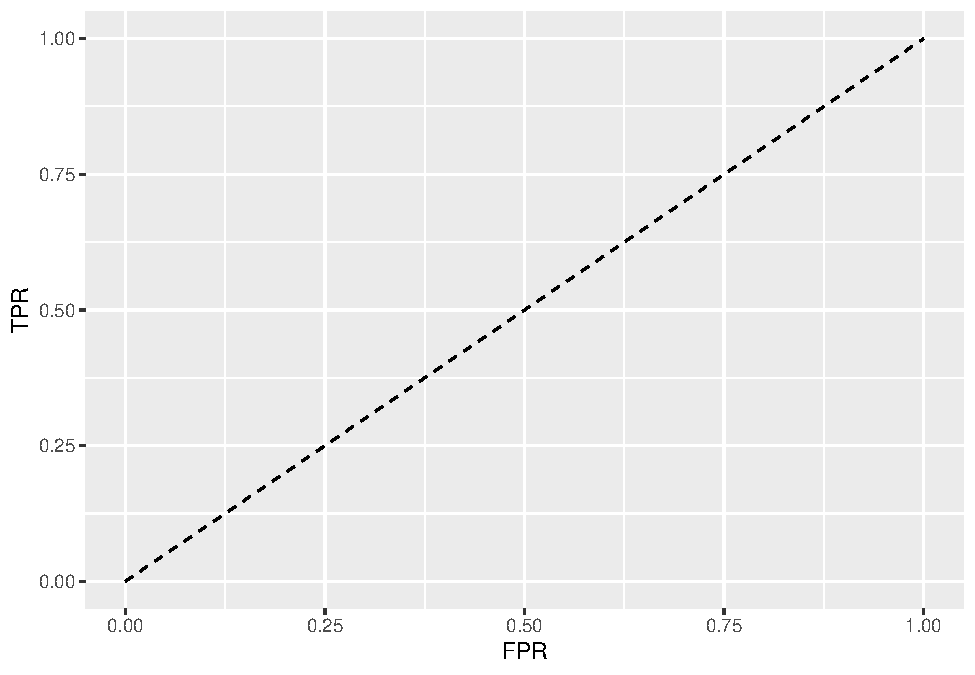
\includegraphics{Project2_files/figure-latex/unnamed-chunk-17-1.pdf}

\begin{Shaded}
\begin{Highlighting}[]
\NormalTok{ROC1<-ROC1[}\KeywordTok{order}\NormalTok{(}\OperatorTok{-}\NormalTok{ROC1}\OperatorTok{$}\NormalTok{cutoff),]}
\NormalTok{widths<-}\KeywordTok{diff}\NormalTok{(ROC1}\OperatorTok{$}\NormalTok{FPR)}
\NormalTok{heights<-}\KeywordTok{vector}\NormalTok{()}
\ControlFlowTok{for}\NormalTok{(i }\ControlFlowTok{in} \DecValTok{1}\OperatorTok{:}\DecValTok{100}\NormalTok{) heights[i]<-ROC1}\OperatorTok{$}\NormalTok{TPR[i]}\OperatorTok{+}\NormalTok{ROC1}\OperatorTok{$}\NormalTok{TPR[i}\OperatorTok{+}\DecValTok{1}\NormalTok{]}
\NormalTok{AUC<-}\KeywordTok{sum}\NormalTok{(heights}\OperatorTok{*}\NormalTok{widths}\OperatorTok{/}\DecValTok{2}\NormalTok{)}
\NormalTok{AUC}\OperatorTok\KeywordTok{round}\NormalTok{(}\DecValTok{3}\NormalTok{)}
\end{Highlighting}
\end{Shaded}

\begin{verbatim}
## [1] NaN
\end{verbatim}

\emph{Here the ROC is shown, and the AUC is calculated using the loop
for ranks. The AUC is 0.623, which is actually categorized as a poor
AUC.}

\begin{Shaded}
\begin{Highlighting}[]
\NormalTok{class_diag<-}\ControlFlowTok{function}\NormalTok{(probs,truth)\{}
\NormalTok{ tab<-}\KeywordTok{table}\NormalTok{(}\KeywordTok{factor}\NormalTok{(probs}\OperatorTok{>}\NormalTok{.}\DecValTok{5}\NormalTok{,}\DataTypeTok{levels=}\KeywordTok{c}\NormalTok{(}\StringTok{"FALSE"}\NormalTok{,}\StringTok{"TRUE"}\NormalTok{)),truth)}
\NormalTok{ acc=}\KeywordTok{sum}\NormalTok{(}\KeywordTok{diag}\NormalTok{(tab))}\OperatorTok{/}\KeywordTok{sum}\NormalTok{(tab)}
\NormalTok{ sens=tab[}\DecValTok{2}\NormalTok{,}\DecValTok{2}\NormalTok{]}\OperatorTok{/}\KeywordTok{colSums}\NormalTok{(tab)[}\DecValTok{2}\NormalTok{]}
\NormalTok{ spec=tab[}\DecValTok{1}\NormalTok{,}\DecValTok{1}\NormalTok{]}\OperatorTok{/}\KeywordTok{colSums}\NormalTok{(tab)[}\DecValTok{1}\NormalTok{]}
\NormalTok{ ppv=tab[}\DecValTok{2}\NormalTok{,}\DecValTok{2}\NormalTok{]}\OperatorTok{/}\KeywordTok{rowSums}\NormalTok{(tab)[}\DecValTok{2}\NormalTok{]}
 \ControlFlowTok{if}\NormalTok{(}\KeywordTok{is.numeric}\NormalTok{(truth)}\OperatorTok{==}\OtherTok{FALSE} \OperatorTok{&}\StringTok{ }\KeywordTok{is.logical}\NormalTok{(truth)}\OperatorTok{==}\OtherTok{FALSE}\NormalTok{) truth<-}\KeywordTok{as.numeric}\NormalTok{(truth)}\OperatorTok{-}\DecValTok{1}
 
\NormalTok{ ord<-}\KeywordTok{order}\NormalTok{(probs, }\DataTypeTok{decreasing=}\OtherTok{TRUE}\NormalTok{)}
\NormalTok{ probs <-}\StringTok{ }\NormalTok{probs[ord]; truth <-}\StringTok{ }\NormalTok{truth[ord]}
\NormalTok{ TPR=}\KeywordTok{cumsum}\NormalTok{(truth)}\OperatorTok{/}\KeywordTok{max}\NormalTok{(}\DecValTok{1}\NormalTok{,}\KeywordTok{sum}\NormalTok{(truth))}
\NormalTok{ FPR=}\KeywordTok{cumsum}\NormalTok{(}\OperatorTok{!}\NormalTok{truth)}\OperatorTok{/}\KeywordTok{max}\NormalTok{(}\DecValTok{1}\NormalTok{,}\KeywordTok{sum}\NormalTok{(}\OperatorTok{!}\NormalTok{truth))}
\NormalTok{ dup<-}\KeywordTok{c}\NormalTok{(probs[}\OperatorTok{-}\DecValTok{1}\NormalTok{]}\OperatorTok{>=}\NormalTok{probs[}\OperatorTok{-}\KeywordTok{length}\NormalTok{(probs)], }\OtherTok{FALSE}\NormalTok{)}
\NormalTok{ TPR<-}\KeywordTok{c}\NormalTok{(}\DecValTok{0}\NormalTok{,TPR[}\OperatorTok{!}\NormalTok{dup],}\DecValTok{1}\NormalTok{); FPR<-}\KeywordTok{c}\NormalTok{(}\DecValTok{0}\NormalTok{,FPR[}\OperatorTok{!}\NormalTok{dup],}\DecValTok{1}\NormalTok{)}
\NormalTok{ n <-}\StringTok{ }\KeywordTok{length}\NormalTok{(TPR)}
\NormalTok{ auc<-}\StringTok{ }\KeywordTok{sum}\NormalTok{( ((TPR[}\OperatorTok{-}\DecValTok{1}\NormalTok{]}\OperatorTok{+}\NormalTok{TPR[}\OperatorTok{-}\NormalTok{n])}\OperatorTok{/}\DecValTok{2}\NormalTok{) }\OperatorTok{*}\StringTok{ }\NormalTok{(FPR[}\OperatorTok{-}\DecValTok{1}\NormalTok{]}\OperatorTok{-}\NormalTok{FPR[}\OperatorTok{-}\NormalTok{n]) )}
 \KeywordTok{data.frame}\NormalTok{(acc,sens,spec,ppv,auc)}
\NormalTok{\} }

\KeywordTok{set.seed}\NormalTok{(}\DecValTok{1234}\NormalTok{)}
\NormalTok{k=}\DecValTok{10} 
\NormalTok{data1<-melanoma[}\KeywordTok{sample}\NormalTok{(}\KeywordTok{nrow}\NormalTok{(melanoma)),] }\CommentTok{#randomly order rows}
\NormalTok{folds<-}\KeywordTok{cut}\NormalTok{(}\KeywordTok{seq}\NormalTok{(}\DecValTok{1}\OperatorTok{:}\KeywordTok{nrow}\NormalTok{(melanoma)),}\DataTypeTok{breaks=}\NormalTok{k,}\DataTypeTok{labels=}\NormalTok{F) }\CommentTok{#create folds}
\NormalTok{diags<-}\OtherTok{NULL}
\ControlFlowTok{for}\NormalTok{(i }\ControlFlowTok{in} \DecValTok{1}\OperatorTok{:}\NormalTok{k)\{}
\NormalTok{ train<-data1[folds}\OperatorTok{!=}\NormalTok{i,]}
\NormalTok{ test<-data1[folds}\OperatorTok{==}\NormalTok{i,]}
\NormalTok{ truth<-test}\OperatorTok{$}\NormalTok{y}
 
 \CommentTok{#fit<-glm(y~thickness + age,data=train,family="binomial")}
 \CommentTok{#probs<-predict(fit,newdata = test,type="response")}
 
 \CommentTok{#diags<-rbind(diags,class_diag(probs,truth))}
\NormalTok{\}}

\CommentTok{#apply(diags,2,mean)}
\end{Highlighting}
\end{Shaded}

\emph{Using a 10-fold cross validation test, the AUC decreased to 0.582,
which is now classified as bad. The accuracy is 0.617, the sensitivity
is 0.091, the specificity is 0.948, and the recall is not applicable.}

\textbf{LASSO MODEL}

\begin{Shaded}
\begin{Highlighting}[]
\CommentTok{#library(glmnet)}
\KeywordTok{data}\NormalTok{(}\StringTok{"melanoma"}\NormalTok{)}
\NormalTok{y<-}\KeywordTok{as.matrix}\NormalTok{(melanoma}\OperatorTok{$}\NormalTok{y)}
\NormalTok{x<-melanoma}\OperatorTok\NormalTok{dplyr}\OperatorTok{::}\KeywordTok{select}\NormalTok{(time}\OperatorTok{:}\NormalTok{ulcer)}\OperatorTok\KeywordTok{mutate_all}\NormalTok{(scale)}\OperatorTok\NormalTok{as.matrix}
\CommentTok{#cv<-cv.glmnet(x,y)}

\CommentTok{#lasso1<-glmnet(x,y,lambda=cv$lambda.1se)}
\CommentTok{#coef(lasso1)}
\end{Highlighting}
\end{Shaded}

\emph{This LASSO model shows that the year variable is the only
significant predictor of the status of the patient after the melanoma
removal surgery-whether they lived or died of melanoma.}

\begin{Shaded}
\begin{Highlighting}[]
\NormalTok{melanoma<-melanoma}\OperatorTok\StringTok{ }\KeywordTok{mutate}\NormalTok{(}\DataTypeTok{y=}\KeywordTok{ifelse}\NormalTok{(melanoma}\OperatorTok{$}\NormalTok{status}\OperatorTok{==}\DecValTok{2}\NormalTok{,}\DecValTok{1}\NormalTok{,}\DecValTok{0}\NormalTok{))}

\CommentTok{#set.seed(1234)}
\CommentTok{#k=5 }
\CommentTok{#data1<-melanoma[sample(nrow(melanoma)),] }
\CommentTok{#folds<-cut(seq(1:nrow(mtcars)),breaks=k,labels=F) }
\CommentTok{#diags<-NULL}
\CommentTok{#for(i in 1:k)\{}
 \CommentTok{#train<-data1[folds!=i,]}
 \CommentTok{#test<-data1[folds==i,]}
 \CommentTok{#fit<-lm(y~.,data=train)}
 \CommentTok{#yhat<-predict(fit,newdata=test)}
 \CommentTok{#diags<-mean((test$y-yhat)^2)\}}
\CommentTok{#mean(diags)}
\end{Highlighting}
\end{Shaded}

\emph{The CV's result was 0.049.}


\end{document}
